\documentclass[../calc1-main.tex]{subfiles}

\begin{document}

The best line approximating the graph of $y=f(x)$ near $(a, f(a))$ is the tangent line through $(a, f(a))$.

\begin{figure}[H]
  \centering
  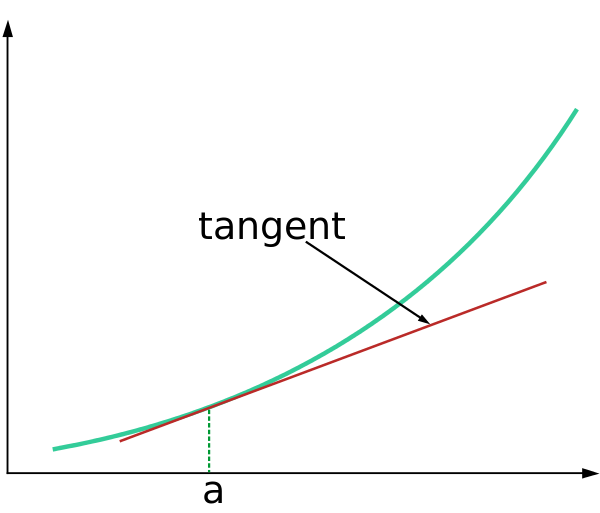
\includegraphics[width=0.25\textwidth]{figures/4-7-lin-approx.png}
\end{figure}

The linearization of the function $f$ about $a$ is the function $L$ defined by
\[
  L(x) = f(a) + f'(a)(x-a)
\]

We say that $L$ approximates $f$ near $x=a$ and write $f(x) \approx L(x)$.

\begin{example}
  Using the linearization, approximate $\sqrt{26}$. (Hint: use the linearization of $\sqrt{x}$ at $x=25$.)
\end{example}
\begin{solution}
  $f'(x) = \frac{1}{2\sqrt{x}}$. $f'(25) = \frac{1}{10}$. So
  \[
    L(x) = 5 + \frac{1}{10} (x-25).
  \]
  Hence $f(26) \approx f(26) = 5.1$.
\end{solution}

\begin{example}
  Approximate $\cos \pi/5 = \cos 36^{\circ}$ using the linearization of $\cos x$ at $x=\pi/6$.
\end{example}

\begin{solution}
  $L(x) = \cos\frac{\pi}{6} - \sin \frac{\pi}{6}(x-\frac{\pi}{6}) = \frac{\sqrt{3}}{2} - \frac{1}{2}(x-\frac{\pi}{6})$.

  \[
    \cos 36^{\circ} \approx L(\pi/5) = \frac{\sqrt{3}}{2} - \frac{1}{2} \frac{\pi}{30} \approx 0.81367
  \]
\end{solution}

\subsection*{Error Estimation}
The error in the linear approximation is
\[
  \frac{f''(s)}{2}(x-a)^2
\]
where $s$ is some number between $a$ and $x$. (The proof depends on the generalized mean value theorem.)

Since we do not know $s$, we have to choose $f''(s)$ to be largest (in absolute value) possible value, to get the maximum error.

So for the previous example, $f''(x) = -\sin x$, $a=\pi/6$, $x=\pi/5$, $\pi/6<s<\pi/5$. Note that $f''(s) \le 1$. So the error is smaller that $\frac{1}{2}(x-a)^2 = \frac{\pi^2}{1800}<0.00549$. So $0.81367 -0.00549 < \cos \pi/5 < 0.81367 + 0.00549$.

\rule{\textwidth}{1pt}
\begin{multicols}{2}
\begin{exercise}
~\\
  \begin{enumerate}
    \item Sketch $y=\frac{1}{\sqrt{x}}$ and its linearization about $x=4$.
    \item Approximate $\sqrt{50}$ using linearization.

    Answer: $7+ \frac{1}{14}$.
    \item Approximate $\sin 46^{\circ}$ using linearization.

    Answer: $\frac{\sqrt{2}}{2} + \frac{\sqrt{2}}{2} \frac{\pi}{180}$. (Note: $f(x) = \sin x^{\circ} = \sin \frac{\pi x}{180}$)
  \end{enumerate}
\end{exercise}
\end{multicols}
\rule{\textwidth}{1pt}

\end{document}
